\documentclass[NET,english,aspectratio=169,notitleframe]{tumbeamer}
%settings
\usepackage[utf8]{inputenc}
\usepackage{pgfplotstable}
\usepackage{marvosym}
\usepackage{filecontents}
\usepackage{packages}
\usepackage{beamermods}

\usepackage[backend=bibtex, style=ieee]{biblatex}

\usepackage{csquotes}
\usepackage{amssymb}% http://ctan.org/pkg/amssymb
\usepackage{pifont}% http://ctan.org/pkg/pifont
\usepackage{booktabs,caption}
\usepackage{threeparttable}
\newcommand{\cmark}{\textcolor{TUMDarkGreen}{\ding{51}}}%
\newcommand{\xmark}{\textcolor{TUMDarkRed}{\ding{55}}}%

\usetikzlibrary{calc}
\usetikzlibrary{arrows.meta}


% For lecture mode (use package option 'lecture'):
%\lecture[GRNVS]{Grundlagen Rechnernetze und Verteilte Systeme}
%\module{IN0010}
%\semester{SoSe\,2016}
%\assistants{Johannes Naab, Stephan Günther, Maurice Leclaire}

\usepackage{pgfplots}
\pgfplotsset{compat=newest}
\usepackage{tumcolor}
\usepackage{tumcolors}
\usepackage{textpos}


\usepackage{pgfpages}
\usepackage{ifthen}
% ============================================================================
% jobname solution
% ============================================================================
\newif\ifsolution%
\ifthenelse{\equal{\detokenize{notes}}{\jobname}}{%
\setbeameroption{show notes on second screen=bottom}
\setbeamercolor{note page}{bg=white, fg=black}
\setbeamercolor{note title}{bg=white!95!black, fg=black}
}{
}

%\xdefinecolor{orange}{cmyk}{0,0.65,0.95,0} 
%\xdefinecolor{dblue}{cmyk}{1,0.54,0.04,0.19}
%\xdefinecolor{blue}{cmyk}{1,0.43,0,0}  
%\xdefinecolor{lblue}{cmyk}{0.65,0.19,0.01,0.04}
%\xdefinecolor{green} {cmyk}{0.35,0,1,0.2} 
%xdefinecolor{yellow}{rgb}{1.00,0.71,0.00} 
%\colorlet{lgtorange}{orange!20} 
%\colorlet{lgtdblue}{dblue!20} 
%\colorlet{lgtblue}{blue!20} 
%\colorlet{lgtlblue}{lblue!20} 
%colorlet{lgtgreen}{green!20} 
%\colorlet{lgtyellow}{yellow!20}

\newcommand\Wider[2][3em]{%
\makebox[\linewidth][c]{%
  \begin{minipage}{\dimexpr\textwidth+#1\relax}
  \raggedright#2
  \end{minipage}%
  }%
}
\usepackage{cancel}
\usepackage{minted}


\addbibresource{lit.bib}


% For beamer mode (default):
 % names of everyone who contributed something, sorted alphabetically
\author[Paul Emmerich, Simon Ellmann]{\textbf{Paul Emmerich}, \textbf{Simon Ellmann}, Fabian Bonk, Alex Egger,\\ Esaú García Sánchez-Torija, Thomas Günzel, Sebastian Di Luzio,\\Alexandru Obada, Maximilian Stadlmeier, Sebastian Voit, Georg Carle}
\title{The Case for Writing Network Drivers in\\ High-Level Programming Languages}
\date{September 24, 2019}

\makeatletter
\let\@@magyar@captionfix\relax
\makeatother

\begin{document}

\setbeamertemplate{footline}{}
  \begin{frame}[c,noframenumbering]
%    \begin{tikzpicture}[overlay,remember picture]
%      \node[opacity=0.5,anchor=south east] at ($(current page.south east)+(-1,-1)$) {%
%    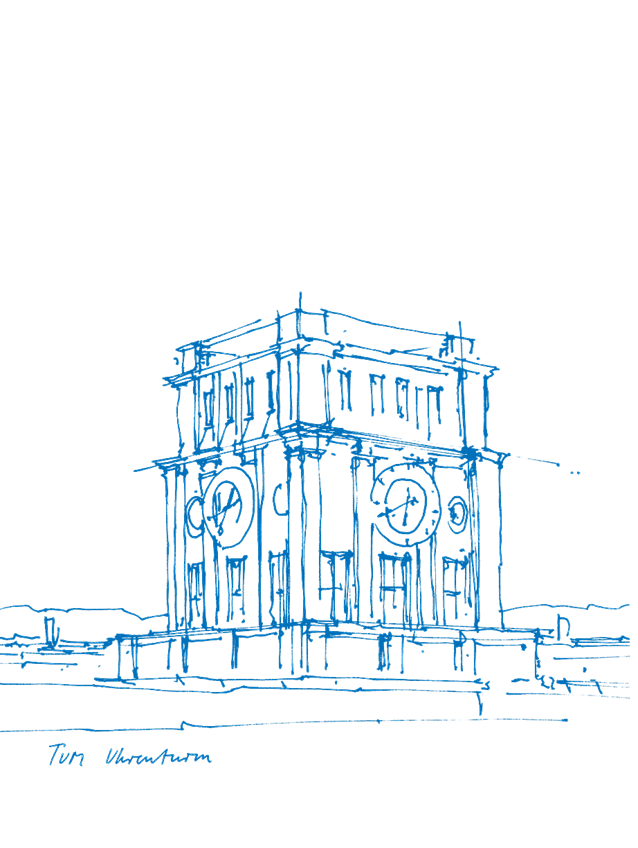
\includegraphics[width=.4\textwidth]{pics/TUM_Uhrenturm.png}};
%  \end{tikzpicture}
  \centering%
  \Large%
  \strut\textcolor{TUMBlue}{\inserttitle}%
  \\[4ex]%
  \normalsize%
\footnotesize  \strut\insertauthor%
  \\[2ex]%
  \footnotesize%
  \insertdate%
  \\[4ex]%
  \ifdefined\departmentname%
    \ifdefined\chairname%
      \chairname\\%
    \fi%
    \departmentname\\%
  \fi%
  \TUMname\\%
\end{frame}
\setbeamertemplate{footline}[tumfootline]

\begin{frame}{C is an awesome language for operating systems!}
\begin{itemize}
\item Low-level access to memory and devices
\item Pointers are awesome
\item Everyone can read and write C
\item You can write safe and secure code if you try really hard
\end{itemize}
\end{frame}


\begin{frame}{C can cause security problems}
\centering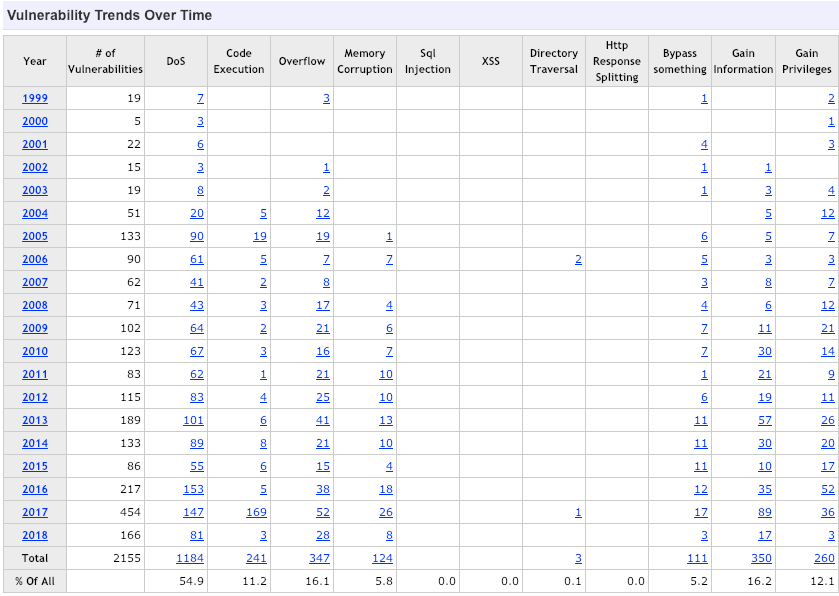
\includegraphics[trim={0 13cm 0 0},clip,width=0.65\textwidth]{pics/cve}

\footnotesize (...)

\centering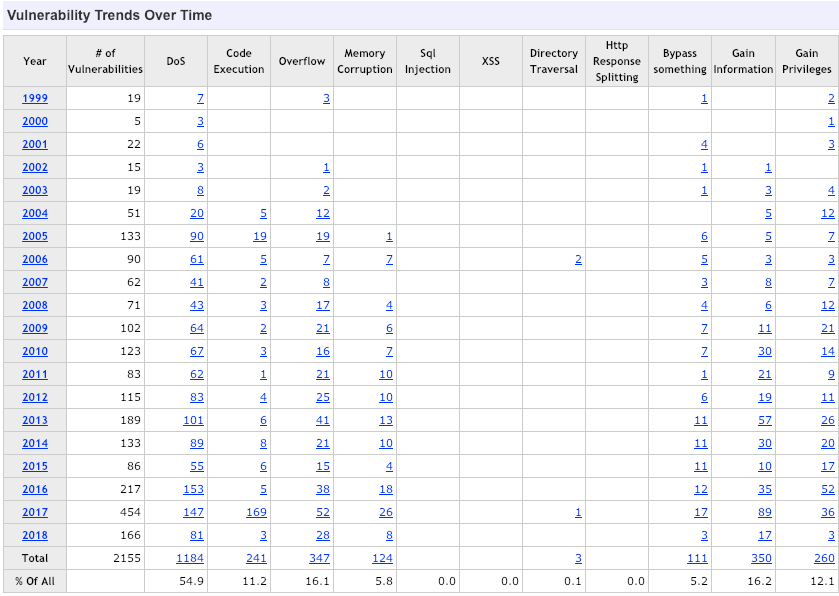
\includegraphics[trim={0 0 0 17.5cm},clip,width=0.65\textwidth]{pics/cve}

\begin{itemize}
\item Screenshot from \url{https://www.cvedetails.com/}
\item Security bugs found in the Linux kernel in the last $\approx$ 20 years
\end{itemize}

\end{frame}


\begin{frame}{C can cause security problems}
\begin{itemize}
\item Not all bugs can be blamed on the language\uncover<2->{, but 61\% can}
\item Cutler et al. analyzed 65 CVEs categorized as code execution in the Linux kernel \footnote{C. Cutler, M. F. Kaashoek, and R. T. Morris, \emph{``The benefits and costs of writing a POSIX kernel in a high-level language''}, USENIX OSDI, 2018}
\end{itemize}
\pause
\begin{table}
\centering
\begin{tabular}{ l  r r l }
  \toprule
  Bug type & Num. & Perc. & Can be avoided by using a better language? \\
  \midrule
  Various & 11 & 17\% & Unclear/Maybe \\
  Logic & 14 & 22\% & No \\
  Use-after-free & 8 & 12\% & Yes \\
  Out of bounds & 32 & 49\% & Yes (likely leads to panic) \\
  \bottomrule  
\end{tabular}
\caption{Code execution vulnerabilities in the Linux kernel identified by Cutler et al.$^1$}
\end{table}
\end{frame}


\begin{frame}{Let's rewrite all operating systems in better languages?}
\begin{itemize}
\item Rewriting the whole operating system in a safer language is a laudable effort
\begin{itemize}
\item Redox (Rust) wants to become a production-grade OS but currently isn't
\item Singularity (Sing\#, Microsoft Research) demonstrated some interesting concepts
\item Biscuit (Go) implements parts of POSIX for research
\item Unikernels like MirageOS (OCaml) or IncludeOS (C++) can be useful in some scenarios
\end{itemize}
\pause
\item But none of these will replace your main operating system any time soon
\end{itemize}
\end{frame}


\begin{frame}{Where are these bugs that could have been prevented?}
\begin{itemize}
\item We looked at these 40 preventable bugs
%\pause
\item 39 of them were in drivers (the other was in the Bluetooth stack)
\pause
\item 13 were in the Qualcomm WiFi driver
\end{itemize}
%\pause
%\centering
\includegraphics[height=0.5\textheight]{pics/surprised_pikachu}
\end{frame}





\begin{frame}{Can we rewrite drivers in better languages?}
\begin{itemize}
\item User space drivers can be written in \emph{any} language!
\item But are all languages an equally good choice?
\item Is a JIT compiler or a garbage collector a problem in a driver?
\end{itemize}
\end{frame}


\begin{frame}{Challenges for high-level languages}
\begin{itemize}
\item Access to \texttt{mmap} with the proper flags
\item Handle externally allocated (foreign) memory in the language
\item Handle memory layouts/formats (i.e., access memory that looks like a given C struct)
\item Memory access semantics: memory barriers, volatile reads/writes
\item Some operations in drivers are inherently unsafe
\end{itemize}
\end{frame}


\begin{frame}{Why look at network drivers?}
\begin{itemize}
\item Easy to benchmark to quantify results
\item Huge attack surface: exposed to the external world by design
\item User space network drivers are already quite common (e.g., DPDK, Snabb)
\item Network stacks are also moving into the user space (e.g., QUIC)
\pause
\item Everything mentioned here is applicable to other drivers as well
\end{itemize}
\end{frame}


\begin{frame}{Network driver complexity is increasing}
\centering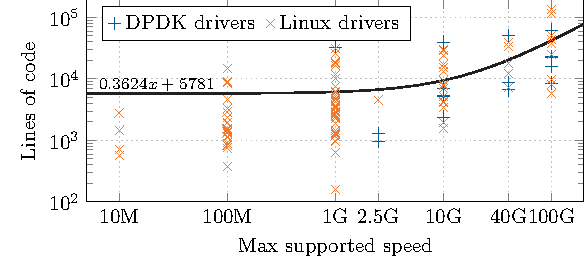
\includegraphics[scale=1.1]{figures/drivers-loc-scatterplot}
\end{frame}





\begin{frame}{We wrote full user space network drivers in these languages}
\begin{figure}
    \centering
    \begin{subfigure}[t]{0.12\textwidth}
        \centering
        \scalebox{1.4}{\Huge C\#}
    \end{subfigure}
    ~ 
    \begin{subfigure}[t]{0.20\textwidth}
        \centering
        
\includegraphics[width=0.88\textwidth]{pics/swift}
    \end{subfigure}
    ~ 
    \begin{subfigure}[t]{0.18\textwidth}
        \centering
        
\includegraphics[width=1.\textwidth]{pics/ocaml}
	\vspace{0.2cm}
    \end{subfigure}
    ~
    \begin{subfigure}[t]{0.15\textwidth}
        \centering
        
\includegraphics[width=0.50\textwidth]{pics/java}
    \end{subfigure}
    ~
    \begin{subfigure}[t]{0.15\textwidth}
        \centering
	\vspace{-1.75cm}
        
\includegraphics[width=0.50\textwidth]{pics/v8}
	\scalebox{1.0}{\Large \textbf{JavaScript}}
    \end{subfigure}
    \\
    \centering
    ~ 
    \begin{subfigure}[t]{0.2\columnwidth}
        \centering
        
\includegraphics[width=0.5\textwidth]{pics/haskell}
    \end{subfigure}
    ~ 
    \begin{subfigure}[t]{0.2\columnwidth}
        \centering
        
\includegraphics[width=0.95\textwidth]{pics/go}
    \end{subfigure}
    ~ 
    \begin{subfigure}[t]{0.2\columnwidth}
        \centering
        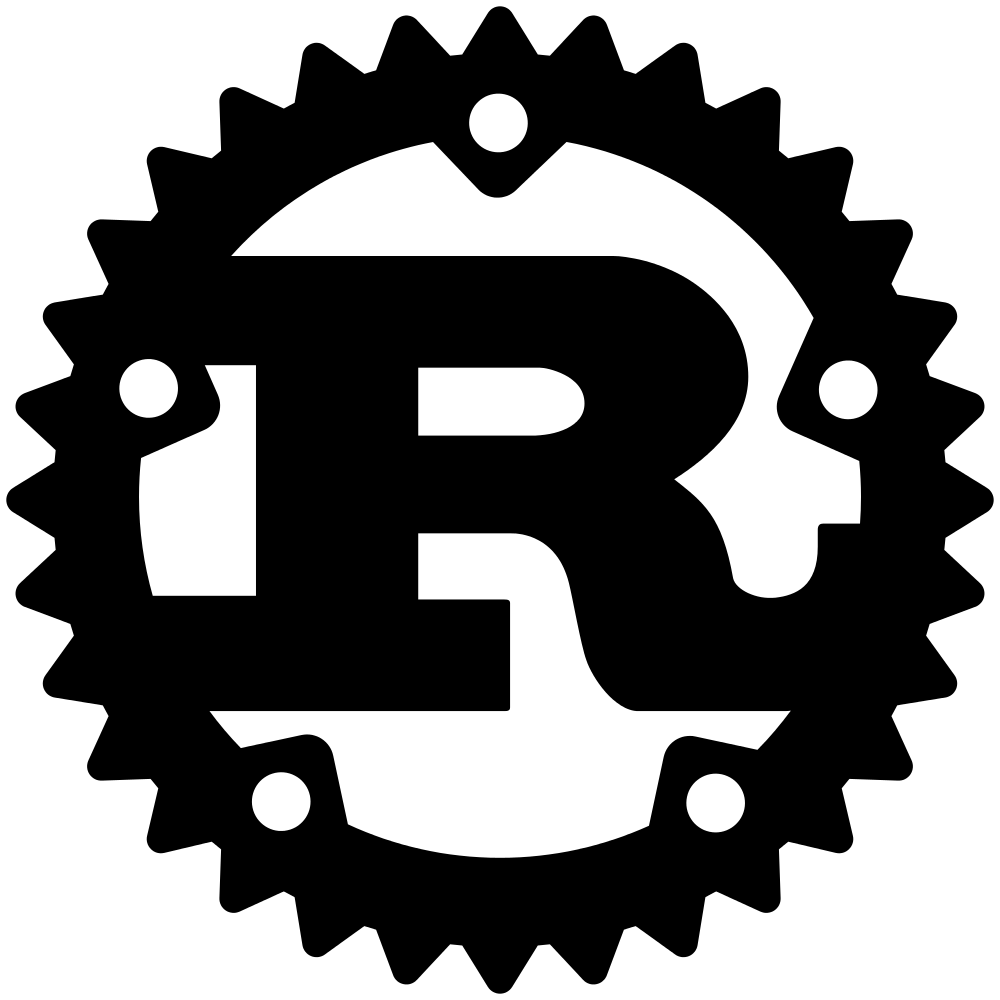
\includegraphics[width=0.45\textwidth]{pics/rust}
    \end{subfigure}
    ~ 
    \begin{subfigure}[t]{0.3\columnwidth}
	\centering
        
\includegraphics[width=0.9\textwidth]{pics/python}
    \end{subfigure}
\end{figure}
\end{frame}

\begin{frame}{Goals for our implementations}
\begin{itemize}
\item Implement the same feature set as our ixy C driver
\item Use a similar structure and architecture as ixy
\item Write idiomatic code for the selected language
\item Use language safety features where possible
\item Quantify trade-offs for performance vs. safety
%\vspace{1em}
%\item This allows us to compare different languages %for safety-critical systems
\end{itemize}
\end{frame}




\setbeamertemplate{footline}{}
\begin{frame}{Language comparison: Safety properties}
\begin{table}[t]
 \setlength{\tabcolsep}{1.3mm}
	\centering
	\footnotesize
	\begin{tabular}{lccccc}
		& \multicolumn{2}{c}{\textbf{General memory}} & \multicolumn{2}{c}{\hspace{-1em}\textbf{Packet buffers}}  \\
		\textbf{Language} & \textbf{Bounds checks} & \textbf{Use after free}  & \textbf{Bounds checks} & \textbf{Use after free} & \textbf{Int overflows} \\
		\toprule
		C & \xmark & \xmark & \xmark & \xmark & \xmark \\
		Rust & &  &  &  &  \\
		Go  & &  &  &  &  \\
		C\#  & &  &  &  &  \\
		Java & & & & & \\
		OCaml  & &  &  &  &  \\
		Haskell  & &  &  &  &  \\
		Swift  & &  &  &  &  \\
		JavaScript & & & & & \\
		Python  & &  &  &  &  \\
		\bottomrule
	\end{tabular}
	\caption{Language-level protections against classes of bugs in our drivers}
	\label{tbl:lang-safety}
	\vspace{-3em}
\end{table}
\end{frame}
\setbeamertemplate{footline}[tumfootline]

\setbeamertemplate{footline}{}
\begin{frame}{Language comparison: Safety properties}
\begin{table}[t]
 \setlength{\tabcolsep}{1.3mm}
	\centering
	\footnotesize
	\begin{tabular}{lccccc}
		& \multicolumn{2}{c}{\textbf{General memory}} & \multicolumn{2}{c}{\hspace{-1em}\textbf{Packet buffers}}  \\
		\textbf{Language} & \textbf{Bounds checks} & \textbf{Use after free}  & \textbf{Bounds checks} & \textbf{Use after free} & \textbf{Int overflows} \\
		\toprule
		C & \xmark & \xmark & \xmark & \xmark & \xmark \\
		Rust & \cmark & \cmark & (\cmark)$^1$ & \cmark & (\cmark)$^4$ \\
		Go & \cmark & \cmark & (\cmark)$^1$ & (\cmark)$^3$ & \xmark \\
		C\# & \cmark & \cmark & (\cmark)$^1$ & (\cmark)$^3$ & (\cmark)$^4$ \\
		Java & \cmark & \cmark & (\cmark)$^1$ & (\cmark)$^3$ & \xmark \\
		OCaml & \cmark & \cmark & (\cmark)$^1$ & (\cmark)$^3$ & \xmark \\
		Haskell & \cmark & \cmark & (\cmark)$^1$ & (\cmark)$^3$ & (\cmark)$^5$ \\
		Swift & \cmark & \cmark & \xmark$^2$ & (\cmark)$^3$ & \cmark \\
		JavaScript & \cmark & \cmark & (\cmark)$^1$ & (\cmark)$^3$ & (\cmark)$^5$ \\
		Python & \cmark & \cmark & (\cmark)$^1$ & (\cmark)$^3$ & (\cmark)$^5$ \\
		\bottomrule
	\end{tabular}
	\begin{tablenotes}
	\tiny
	\item $^1$ Bounds enforced by wrapper, constructor in unsafe or C code
	\item $^2$ Bounds only enforced in debug mode
	\item $^3$ Buffers are never free'd/gc'd, only returned to a memory pool
	\item $^4$ Disabled by default
	\item $^5$ Uses floating point or arbitrary precision integers by default
	\end{tablenotes}
	\caption{Language-level protections against classes of bugs in our drivers}
	\label{tbl:lang-safety}
	\vspace{-3em}
\end{table}
\end{frame}
\setbeamertemplate{footline}[tumfootline]




\begin{frame}{Performance comparison: Test setup}
%\vspace{-.75cm}
\centering\includestandalone[scale=0.55]{figures/testsetup}
\end{frame}
\setbeamertemplate{footline}[tumfootline]
\setbeamertemplate{headline}[tumheadline]



\begin{frame}{Batching at 3.3\,GHz CPU speed (single core)}
\centering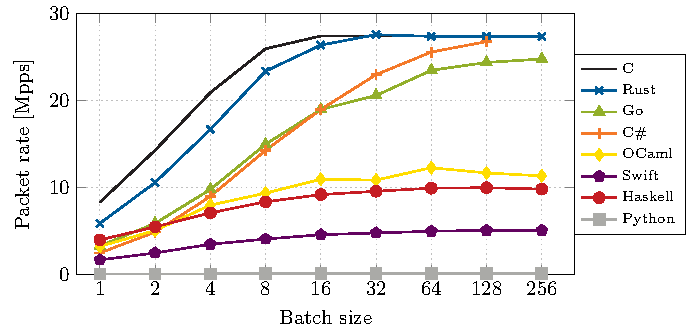
\includegraphics[scale=1]{figures/batches-33.pdf}
\end{frame}


\begin{frame}{Why is Rust slower than C?}
\begin{table}[t]
 \setlength{\tabcolsep}{1.1mm}
	\centering
	\footnotesize
	\begin{tabular}{lrrrrrrrr}
		& \multicolumn{4}{c}{Batch 32, 1.6\,GHz} & \multicolumn{4}{c}{Batch 8, 1.6\,GHz} \\
		\textbf{Events per packet} & \hspace{1em} & \textbf{C} & \textbf{Rust} & \hspace{2.5em} & & \textbf{C} & \textbf{Rust} & \hspace{1.5em} \\
		\toprule
		\textbf{Cycles}                     & & 94 & 100     &&& 108 &  120 \\
		\textbf{Instructions}              & & 127 & 209   &&& 139 &  232  \\
		\textbf{Instr. per cycle}         & & 1.35 & 2.09 &&& 1.29 & 1.93 &  \vspace{0.35em}  \\
		\textbf{Branches}                 & & 18 & 24      &&& 19 &  27  \\
		\textbf{Branch mispredicts} & & 0.05 & 0.08       &&& 0.02 & 0.06 & 		\vspace{0.35em} \\
		\textbf{Store $\mu$ops}       & & 21.8 & 37.4      &&& 24.4 & 43.0  \\
		\textbf{Load $\mu$ops}       & & 30.1 & 77.0      &&& 33.4 & 84.2\  \\
		\textbf{Load L1 hits}                     & & 24.3 & 75.9      &&& 28.8 & 83.1 \\
		\textbf{Load L2 hits}                     & & 1.1 & 0.05         &&& 1.2 & 0.1 \\
		\textbf{Load L3 hits}                     & & 0.9 & 0.0      &&& 0.5 & 0.0 \\
		\textbf{Load L3 misses}               & & 0.3 & 0.1         &&& 0.3 & 0.3 \\
		\bottomrule
	\end{tabular}
	\caption{Performance counter readings in events per packet when forwarding packets}
	\label{tbl:rust-profiling}
	\vspace{-3em}
\end{table}
\end{frame}

\begin{frame}{Why is Rust slower than C?}
\begin{table}[t]
 \setlength{\tabcolsep}{1.1mm}
	\centering
	\footnotesize
	\begin{tabular}{lrrrrrrrr}
		& \multicolumn{4}{c}{Batch 32, 1.6\,GHz} & \multicolumn{4}{c}{\color{TUMLightGray}Batch 8, 1.6\,GHz} \\
		\textbf{Events per packet} & \hspace{1em} & \textbf{C} & \textbf{Rust} & \hspace{2.5em} & & \color{TUMLightGray}\textbf{C} & \color{TUMLightGray}\textbf{Rust} & \hspace{1.5em} \\
		\toprule
		\textbf{Cycles}                     & & 94 & 100     &&& \color{TUMLightGray}{108} &  \color{TUMLightGray}120 \\
		\textbf{Instructions}              & & 127 & 209   &&& \color{TUMLightGray}139 &  \color{TUMLightGray}232  \\
		\textbf{Instr. per cycle}         & & 1.35 & 2.09 &&& \color{TUMLightGray}1.29 & \color{TUMLightGray}1.93 &  \vspace{0.35em}  \\
\color{TUMLightGray}		\textbf{Branches}                 & & \color{TUMLightGray}18 & \color{TUMLightGray}24      &&& \color{TUMLightGray}19 & \color{TUMLightGray} 27  \\
\color{TUMLightGray}		\textbf{Branch mispredicts} & & \color{TUMLightGray}0.05 &\color{TUMLightGray} 0.08       &&&\color{TUMLightGray} 0.02 &\color{TUMLightGray} 0.06 & 		\vspace{0.35em} \\
\color{TUMLightGray}		\textbf{Store $\mu$ops}       & & \color{TUMLightGray}21.8 &\color{TUMLightGray} 37.4      &&&\color{TUMLightGray} 24.4 & \color{TUMLightGray}43.0  \\
\color{TUMLightGray}		\textbf{Load $\mu$ops}       & & \color{TUMLightGray}30.1 &\color{TUMLightGray} 77.0      &&& \color{TUMLightGray}33.4 &\color{TUMLightGray} 84.2\  \\
\color{TUMLightGray}		\textbf{Load L1 hits}                     & & \color{TUMLightGray}24.3 &\color{TUMLightGray} 75.9      &&& \color{TUMLightGray}28.8 & \color{TUMLightGray}83.1 \\
\color{TUMLightGray}		\textbf{Load L2 hits}                     & & \color{TUMLightGray}1.1 &\color{TUMLightGray} 0.05         &&& \color{TUMLightGray}1.2 &\color{TUMLightGray} 0.1 \\
\color{TUMLightGray}		\textbf{Load L3 hits}                     & &\color{TUMLightGray} 0.9 &\color{TUMLightGray} 0.0      &&& \color{TUMLightGray}0.5 & \color{TUMLightGray}0.0 \\
\color{TUMLightGray}		\textbf{Load L3 misses}               & & \color{TUMLightGray}0.3 &\color{TUMLightGray} 0.1         &&& \color{TUMLightGray}0.3 & \color{TUMLightGray}0.3 \\
		\bottomrule
	\end{tabular}
	\caption{Performance counter readings in events per packet when forwarding packets}
	\label{tbl:rust-profiling}
	\vspace{-3em}
\end{table}
\end{frame}





\begin{frame}{Tail latency at 1\,Mpps}
\hspace{1.7cm}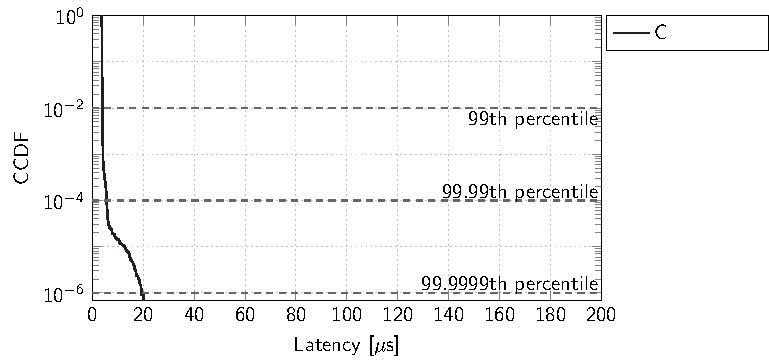
\includegraphics[scale=1]{figures/latency-1/latency-ccdf-1.pdf}
\end{frame}
\addtocounter{framenumber}{-1}

\begin{frame}{Tail latency at 1\,Mpps}
\hspace{1.7cm}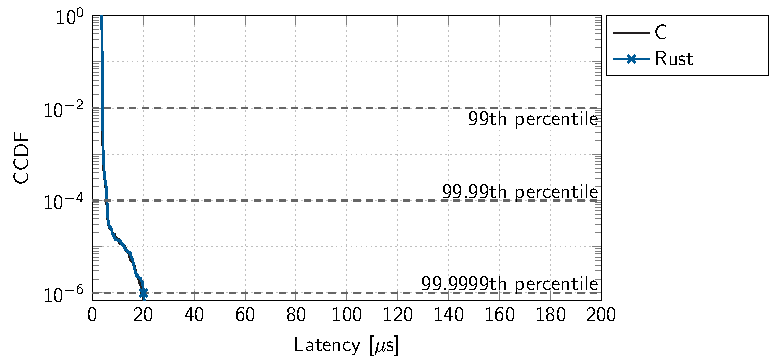
\includegraphics[scale=1]{figures/latency-1/latency-ccdf-2.pdf}
\end{frame}
\addtocounter{framenumber}{-1}

\begin{frame}{Tail latency at 1\,Mpps}
\hspace{1.7cm}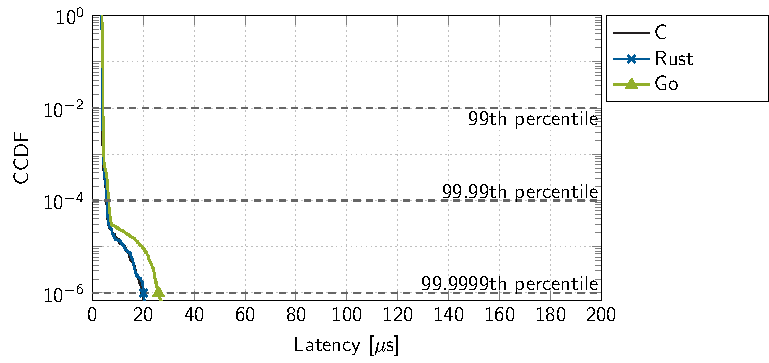
\includegraphics[scale=1]{figures/latency-1/latency-ccdf-3.pdf}
\end{frame}
\addtocounter{framenumber}{-1}

\begin{frame}{Tail latency at 1\,Mpps}
\hspace{1.7cm}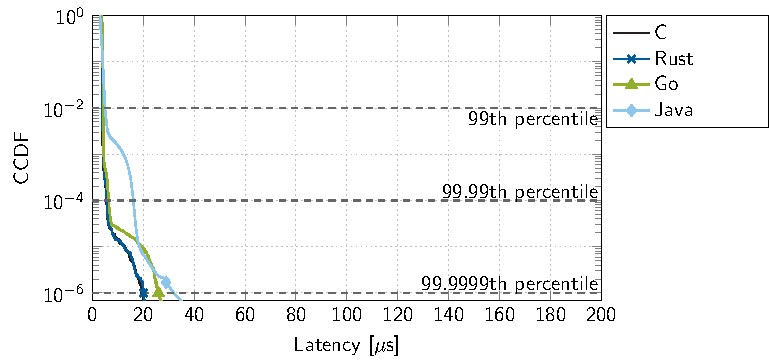
\includegraphics[scale=1]{figures/latency-1/latency-ccdf-4.pdf}
\end{frame}
\addtocounter{framenumber}{-1}

\begin{frame}{Tail latency at 1\,Mpps}
\hspace{1.7cm}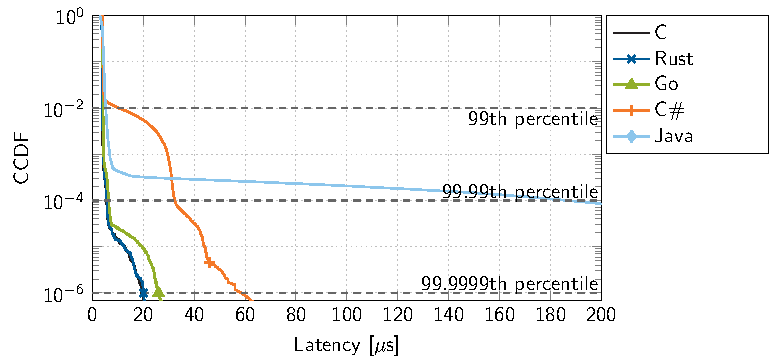
\includegraphics[scale=1]{figures/latency-1/latency-ccdf-5.pdf}
\end{frame}
\addtocounter{framenumber}{-1}

\begin{frame}{Tail latency at 1\,Mpps}
\hspace{1.7cm}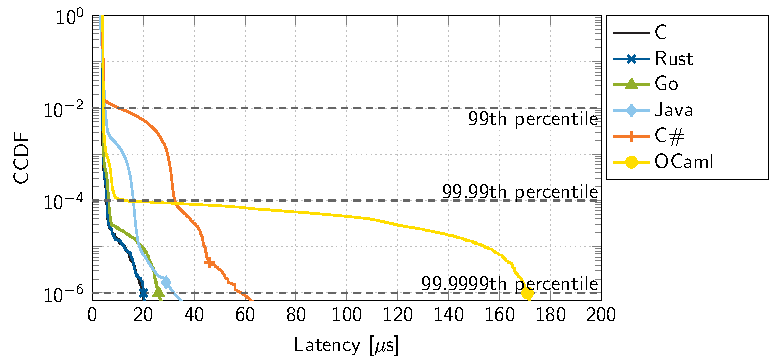
\includegraphics[scale=1]{figures/latency-1/latency-ccdf-6.pdf}
\end{frame}
\addtocounter{framenumber}{-1}

\begin{frame}{Tail latency at 1\,Mpps}
\hspace{1.7cm}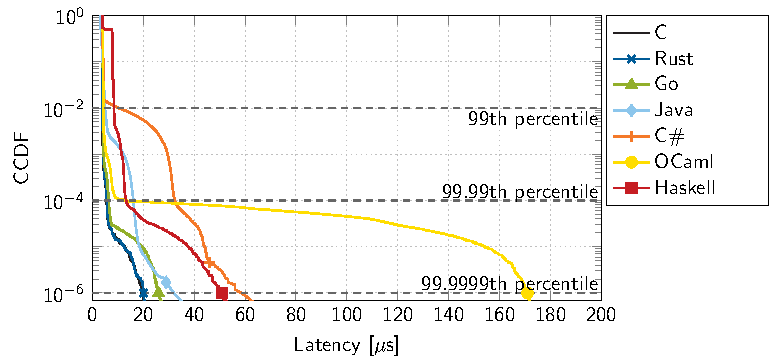
\includegraphics[scale=1]{figures/latency-1/latency-ccdf-7.pdf}
\end{frame}
\addtocounter{framenumber}{-1}

\begin{frame}{Tail latency at 1\,Mpps}
\hspace{1.7cm}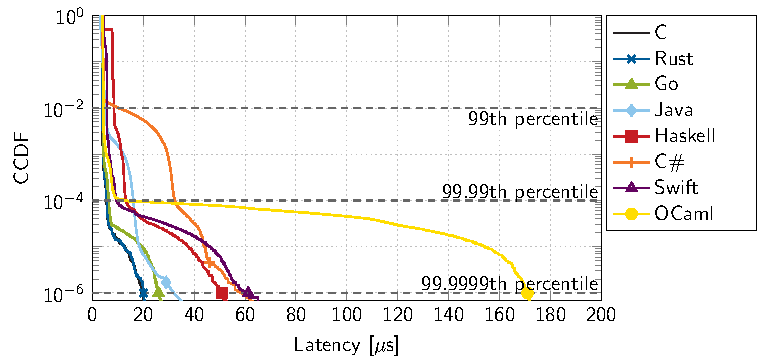
\includegraphics[scale=1]{figures/latency-1/latency-ccdf-8.pdf}
\end{frame}
\addtocounter{framenumber}{-1}

\begin{frame}{Tail latency at 1\,Mpps}
\hspace{1.7cm}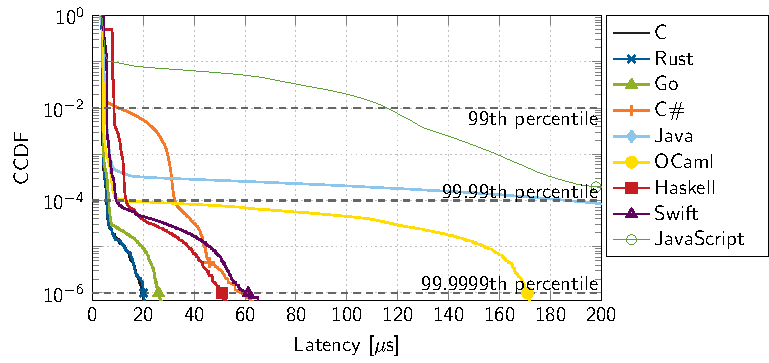
\includegraphics[scale=1]{figures/latency-1/latency-ccdf-9.pdf}
\end{frame}





\begin{frame}{Conclusion: Check out our code}
%\centering \qrcode[height=2cm]{https://github.com/ixy-languages/ixy-languages}
\begin{itemize}
\item Meta-repository with links: \url{https://github.com/ixy-languages/ixy-languages}
\item Should your driver really be in the kernel?
\item Next time you write a driver: consider a user space driver in a cool language
\vspace{1ex}
\item Other cool stuff in the paper: details on implementations, latency at higher loads, Java garbage collector comparison, analysis of user space packet processing frameworks used in academia, study of mistakes made in C, and more...
\end{itemize}
%\centering \Huge Q \& A
\end{frame}

\begin{frame}
\centering\Huge Backup Slides
\end{frame}

\begin{frame}{Languages for code in trustworthy systems}
\begin{itemize}
\item Rust
\begin{itemize}
\item Fast, no garbage collector
\item Low-level: Easy to reason about performance
\item Safest language of the evaluated languages
\end{itemize}
\item Go
\begin{itemize}
\item Fast, low-latency garbage collector
\item Garbage collector tuned for sub-millisecond latency
\item Easier and faster to write than Rust
\end{itemize}
\pause
\item Other languages
\begin{itemize}
\item Implement critical parts in different languages in redundant systems
\item Functional languages for easier formal verification
\end{itemize}
\end{itemize}
\end{frame}

\begin{frame}{Language comparison: Overview}
\begin{table}[t]
 \setlength{\tabcolsep}{2mm}
	\centering
	\footnotesize
	\begin{tabular}{lrrrr}
		\textbf{Language} & \textbf{Main paradigm} & \textbf{Memory management} & \textbf{Compilation} \\
		\toprule
		C & Imperative & No & Compiled \\
		Rust & Imperative & Ownership/RAII & (LLVM) Compiled \\
		Go & Imperative & Garbage collection & Compiled \\
		C\# & Object-oriented & Garbage collection & JIT \\
		Java & Object-oriented & Garbage collection & JIT \\
		OCaml & Functional & Garbage collection & Compiled \\
		Haskell & Functional & Garbage collection & (LLVM) Compiled \\
		Swift & Protocol-oriented & Reference counting & (LLVM) Compiled \\
		JavaScript & Imperative & Garbage collection & JIT \\
		Python & Imperative & Garbage collection & Interpreted \\
		\bottomrule
	\end{tabular}
	\caption{Language overview}
	\label{tbl:languages}
\end{table}
\end{frame}


\setbeamertemplate{footline}{}
\begin{frame}{Language comparison: Implementation sizes}
\begin{table}[t]
 \setlength{\tabcolsep}{2mm}
	\centering
	\footnotesize
	\begin{tabular}{lrrr}
		\\
		\textbf{Lang.} & \textbf{Lines of code}$^1$ & \textbf{Lines of C code}$^1$  & \textbf{Source size (gzip$^2$)} \\
		\toprule
		C & 831 & 831 & 12.9\,kB  \\
		Rust & 961 & 0 & 10.4\,kB\\
		Go & 1640 & 0 & 20.6\,kB \\
		C\# & 1266 & 34 & 13.1\,kB\\
		Java & 2885 & 188 & 31.8\,kB \\
		OCaml & 1177 & 28 &  12.3\,kB\\
		Haskell & 1001 & 0 &  9.6\,kB\\
		Swift & 1506 & 0 & 15.9\,kB \\
		JavaScript & 1004 & 262 &13.0\,kB \\
		Python & 1242 & (Cython) 77 &14.2\,kB \\
		\bottomrule
	\end{tabular}
	\begin{tablenotes}
	\item $^1$ Incl. C code, excluding empty lines and comments, counted with \texttt{cloc}
	\item $^2$ Compression level 6
	\end{tablenotes}
	\caption{Size of our implementations (w/o register constants, stripped features not found in all drivers)}
	\label{tbl:lang-lines}
	\vspace{-3em}
\end{table}
\end{frame}
\setbeamertemplate{footline}[tumfootline]


\end{document}

